\chapter{Results and Conclusions}\label{triumphantDataChapter}

The injection locking was successful and we successfully produced two working beams with an adjustable detuning. We have proven that both beams' frequencies are coupled to and offset from the master laser. Furthermore, the output from the slaves is sufficient to drive the transition. 

First, we see that we can put one slave and the master laser on the spectrum analyzer and scan the master laser and see that the slave scans with it.This is illustrated in Figure\,\ref{fig:slaveMaster}.

\begin{figure}
    %\centerline{\includegraphics[trim=100pt 100pt 100pt 100pt, clip=true, totalheight=0.5\textheight,angle=90]{testfigure}}
    %\centerline{\includegraphics[totalheight=0.3\textheight]{testfigure}}
    \centerline{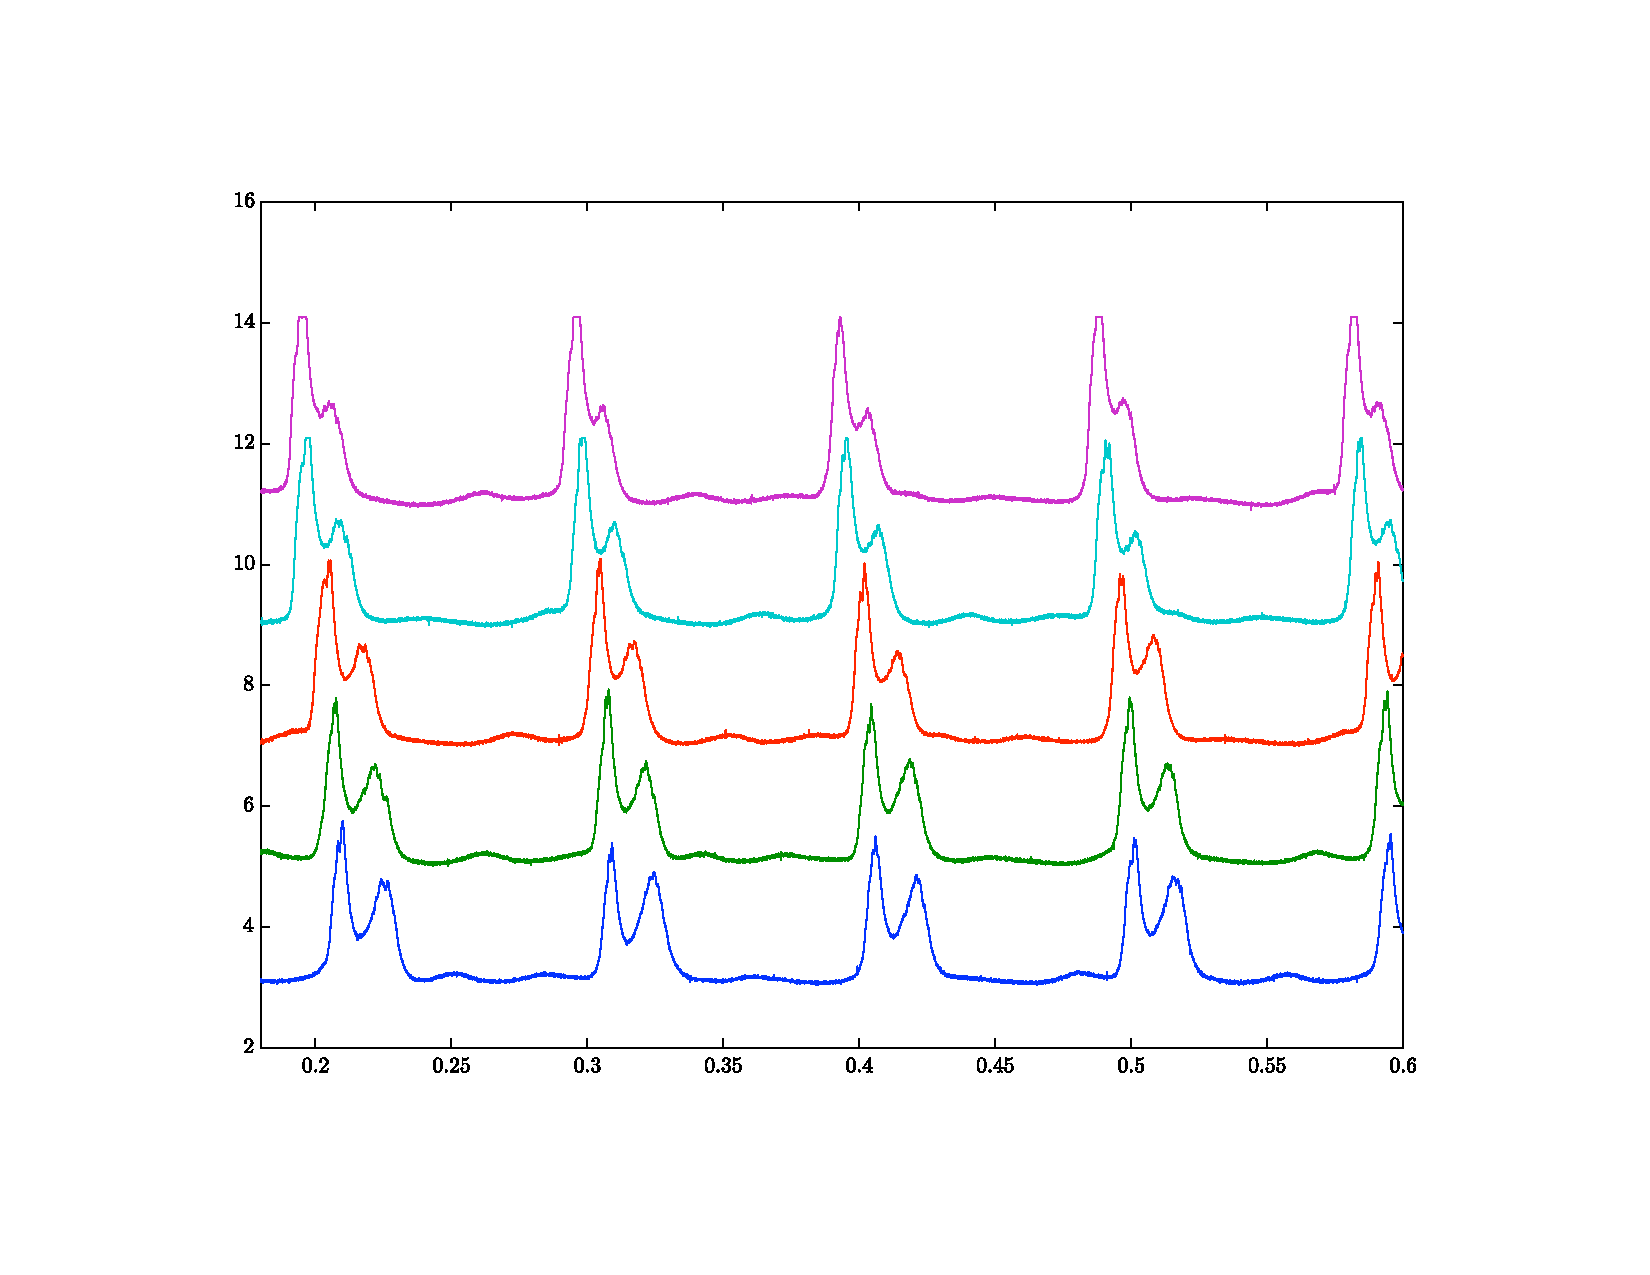
\includegraphics{sampleOffsetData}}
    %\includegraphics[totalheight=0.3\textheight]{testfigure}
    \caption[]{\label{fig:slaveMaster}
    The slave and master laser on the spectrum analyzer. The y axis is the signal on the spectrum analyzer. There are three traces here, each showing the maseter laser at a different frequency. The slave laser is the taller peak, while the other peak belongs to the masdter laser. We can see that the peaks corresponding to the master laser and the slave laser move together.}
\end{figure}

Second, we examined the output of the spectrum analyzer while both slave lasers were coupled into it. 
The two peaks clearly corresponded to the two slave lasers, which we verified by alternatively blocking each of the slaves. 

%We can see that there is a lot of power 


Finally, we performed and experiment where we adjusted the driving frequency of the rf frequency generator driving the AOM. We observed that the peaks on the spectrum analyzer shifted by an amount corresponding to the change in the frequency. This provides strong evidence that the two slaves were injection locked to the modulated beams coming out of the AOM. This data is presented in Figure\,\ref{fig:typicaldata}.

%This test has the further benefit of confirming that we have calculated the free spectral range of the cavity in the spectrum analyzer correctly. 

%where is the energy going? I think it goes from reflecting to transmitting

 
\begin{figure}
    %\centerline{\includegraphics[trim=100pt 100pt 100pt 100pt, clip=true, totalheight=0.5\textheight,angle=90]{testfigure}}
    %\centerline{\includegraphics[totalheight=0.3\textheight]{testfigure}}
    \centerline{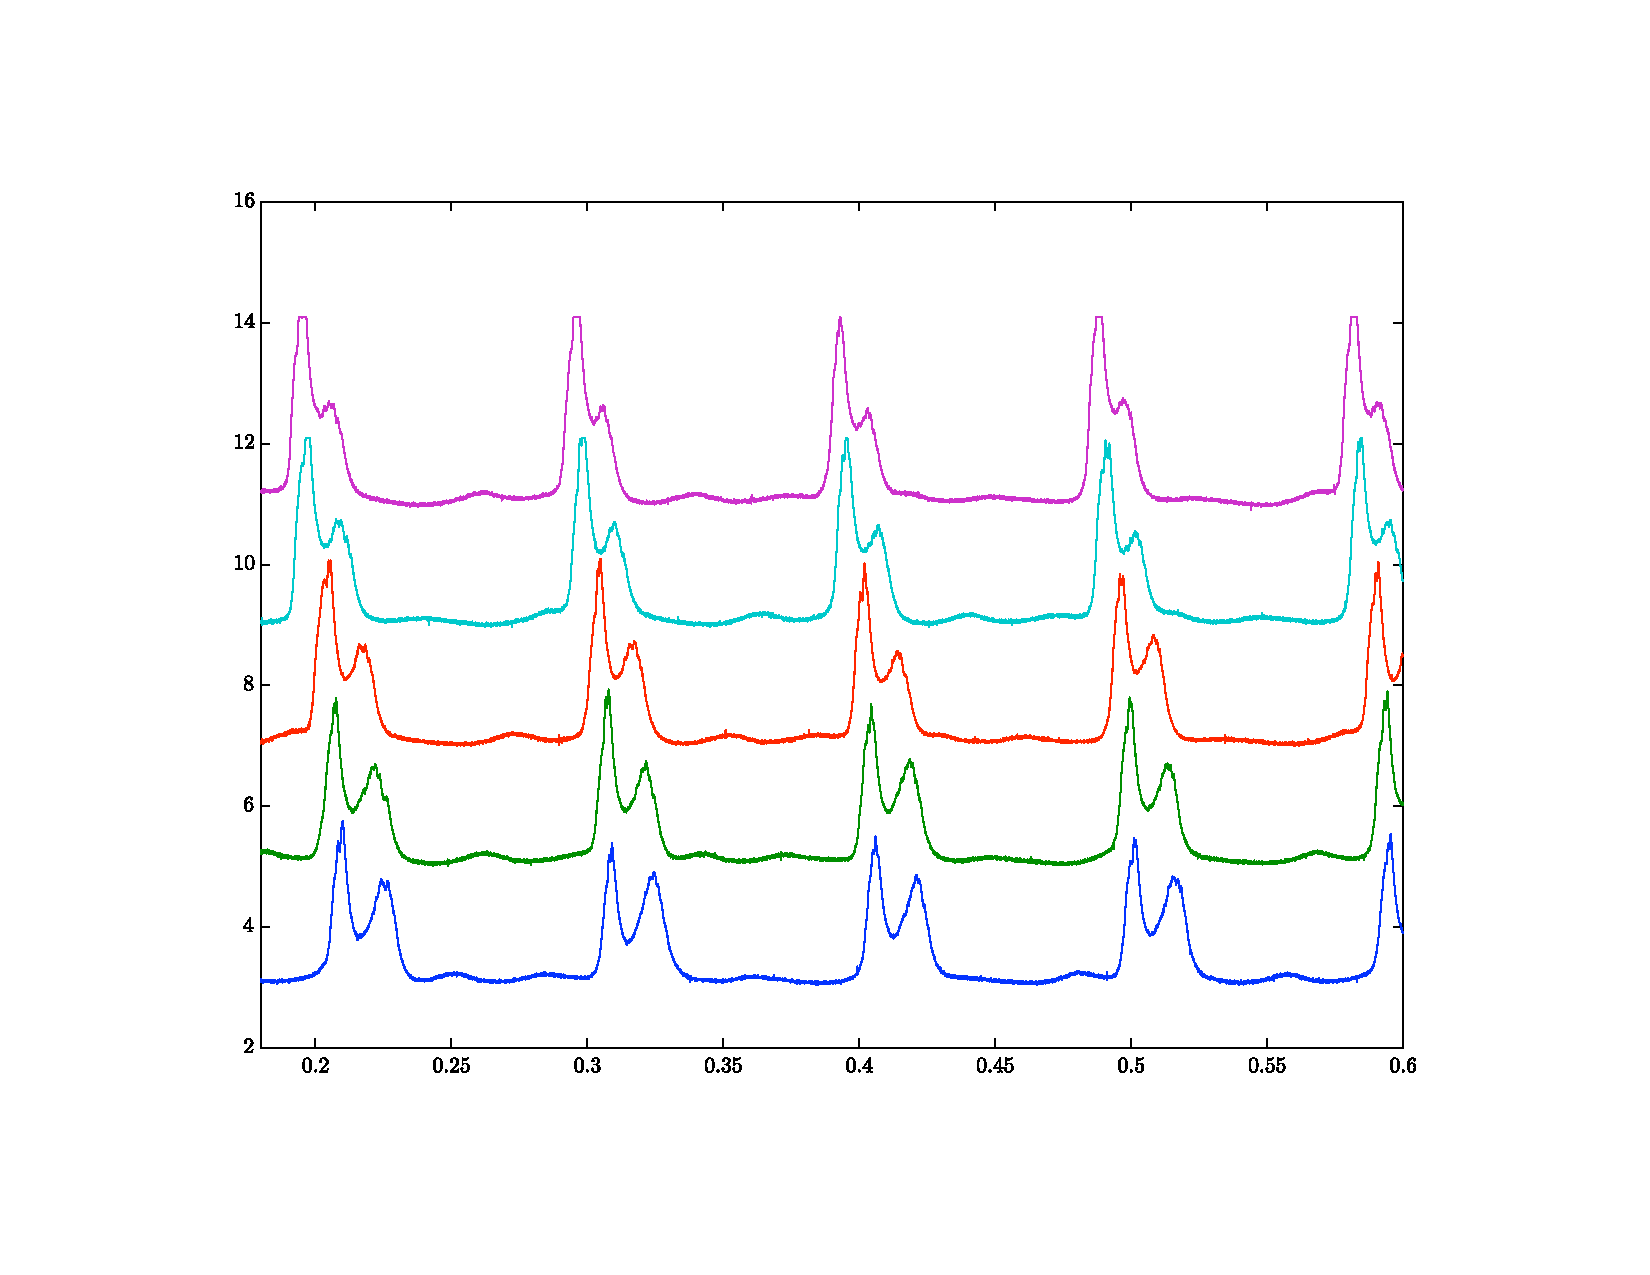
\includegraphics{sampleOffsetData}}
    %\includegraphics[totalheight=0.3\textheight]{testfigure}
    \caption[]{\label{fig:typicaldata}
    We changed the detuning on our frequency generator in 10 MHz increments. These are some of the data that we have that show the spacing between our peaks changing in a predictable way.}
\end{figure}

\begin{figure}
\centerline{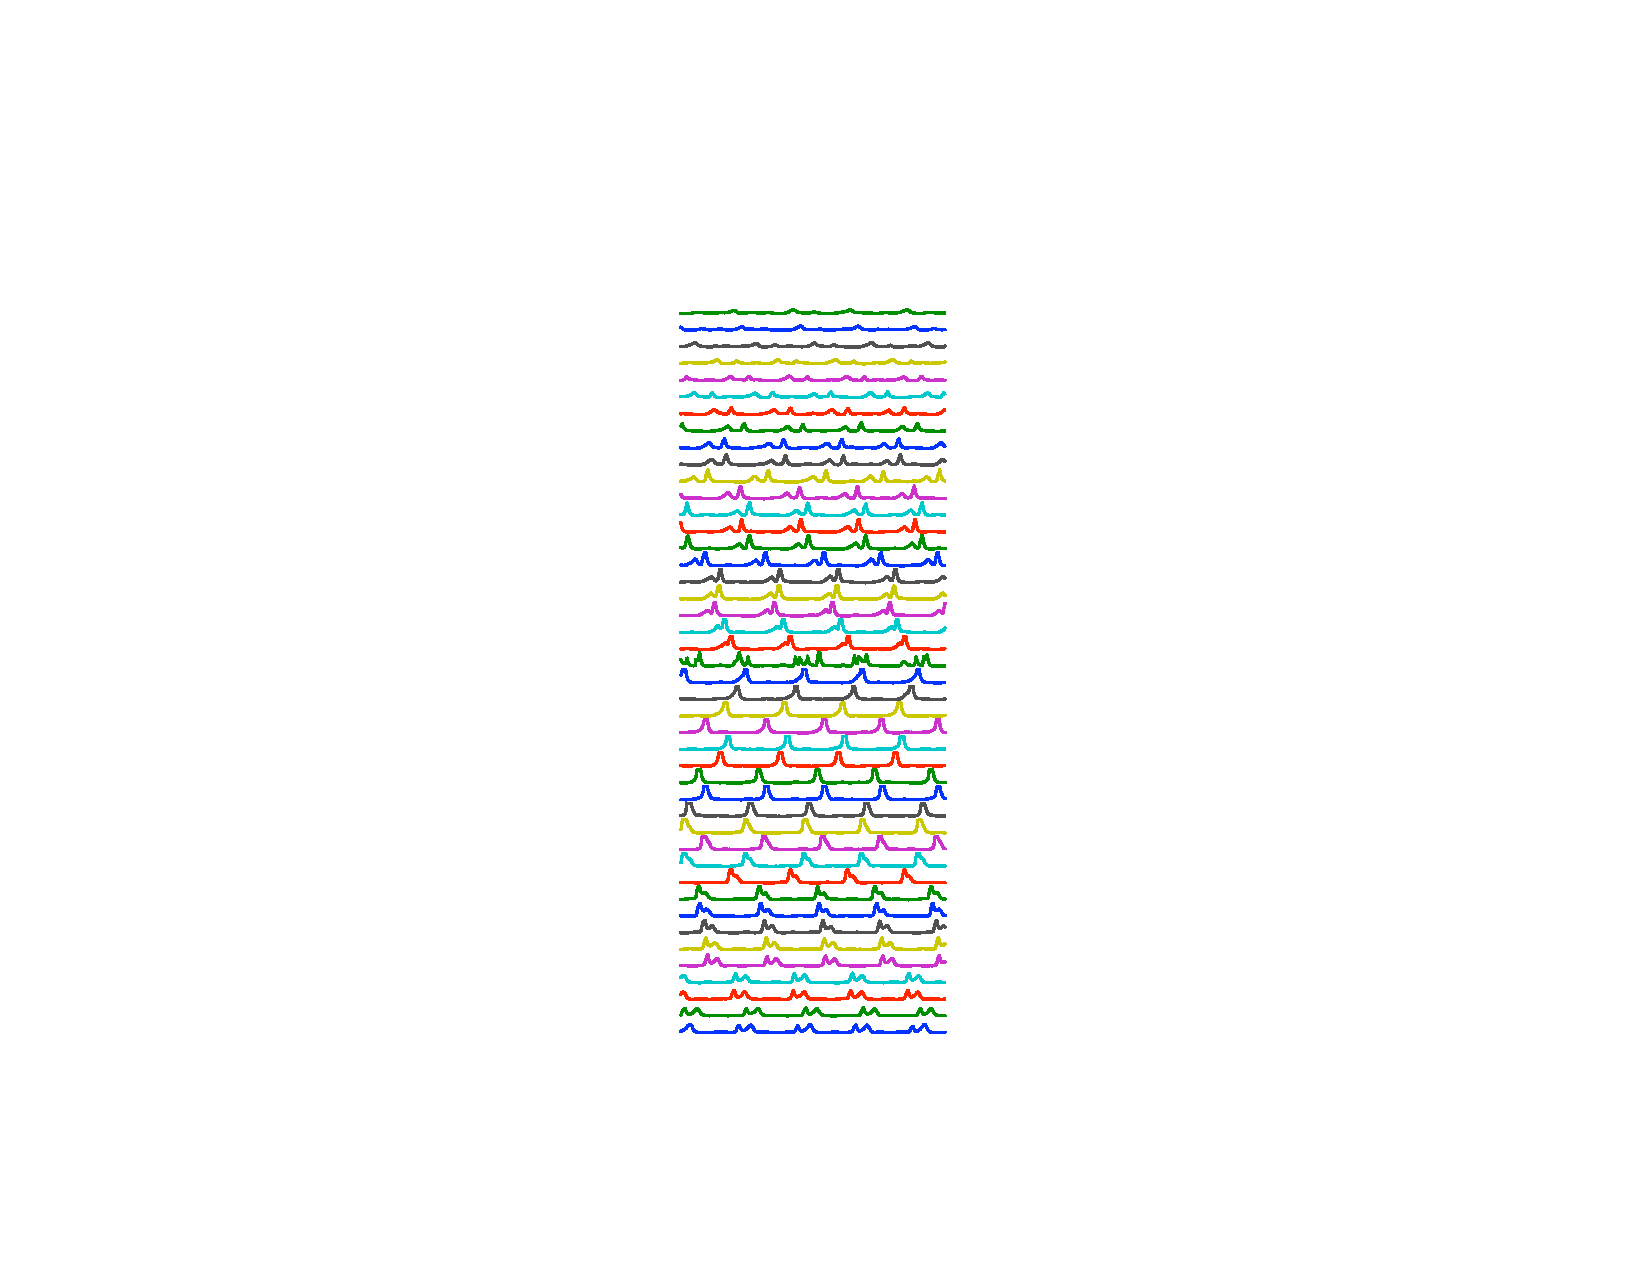
\includegraphics{all_splittingData}}
\caption[]{\label{fig:alldata} 
Spectrum analyzer data for }
\end{figure}

%Also, I have data that I can analyze to examine the feasibility of a Chu lock. I recorded 999 traces that showed the output of the spectrum analyzer, the current and the voltage. I recorded these over several hours, during which the laser drifted into and out of good, single mode operation. In principle, this data could be analyzed. 

We have shown that we can change the oscillator frequency and thereby change the detuning. There are two limiting factors on the extent that we can do this. (Notice in Fig.\ \ref{fig:alldata} that the peaks get small as we continue to detune.) Both factors are geometrical in nature: First, the AOM diffraction efficiency decreases because the Bragg angle changes. Second, the diffraction angle changes, leading to a misalignment of the injected beams and a weakening of injection. However, even for large detunings, the injection lock can be achieved simply by realigning the output beams. We demonstrated this by successfully tuning the AOM driving frequency to the point where injection was lost, realigning (using the lasers as photodiodes) and then reachieving successful injection lock.


